\documentclass[a4paper]{article}

% lang
\usepackage[utf8]{inputenc}   
\usepackage[T1]{fontenc}      
\usepackage[francais]{babel}  

\usepackage{url}
\usepackage{listings}
\lstset{language=python}

%\usepackage{todonotes}
\usepackage[disable]{todonotes}

%graphics
\graphicspath{{Pictures/}}

\usepackage[a4paper]{geometry}

\title{Extension du langage Pythran pour le module \texttt{itertools}}           
\author{Alan Raynaud}
\date{}                      

\sloppy 

\begin{document}

%Page de garde

\maketitle   

\listoftodos[Liste de ce qui est tout doux]

\clearpage

\section*{Le langage pythran}

\subsection*{Amélioration des performances du python}

Le langage python, populaire des les milieux scientifiques, a
l'inconvénient d'être très peu performant comparé à des langages comme
C ou C++. C'est dans le but de permettre d'écrire des programmes
scientifiques en python qui soient les plus performants possible
qu'est né le projet pythran.

Pythran convertit un code python 2.7 en C++, pour ensuite le compiler
en un programme natif hautement performant. L'utilisation de pythran
ne nécessite pas de modification du code existant, seules quelques
annotations de typage sont à ajouter en début de fichiers. Pythran
peut également permettre de paralléliser le code en utilisant des
annotation openMP, classiquement utilisées en C/C++.

Pythran est principalement destiné à être utilisé pour le calcul
scientifique, et ne supporte qu'une sous-partie de python. Le gain de
performance pour ce type de programme peut par contre atteindre un
facteur 2000.

\subsection*{Pythran et ses concurrents}

Il existe de nombreux outils visant à améliorer les performances de
programmes écrits en python.

Il existe par exemple des bibliothèques de calcul scientifique écrites
en C/C++ et destinées à être utilisées depuis python, comme NumPy. Ce
type de bibliothèque n'est pas en concurrence, mais peu au contraire
être complémentaire à pythran.

D'autres approches sont par contre directement en concurrence avec
pythran comme PyPy, Cython ou Shedskin. Ces derniers supportent une
plus grande partie de python que pythran, mais sont moins performant
que pythran pour le calcul scientifique.


\section*{Le problème d'allocation de mémoire inutile}

\subsection*{Description du problème}

Lorsque l'on veut manipuler une grande quantité de données, le plus
simple et de réserver un espace mémoire dans lequel on va les stocker,
pour pouvoir ultérieurement venir les utiliser. L'utilisation que l'on
va en faire varie, mais il est des cas dans lesquels on ne va venir
lire qu'une seule fois chaque donnée.

Plutôt que de produire toutes ces données en une seule fois et les
stocker dans un grand espace, on pourrait les produire, les lire et
les oublier au fur et à mesure. On n'aurait alors besoin que de
réserver l'espace nécessaire à stocker une seule donnée.

Des tests montre qu'en plus de consommer inutilement de la mémoire,
cette sur-allocation d'espace a un coût en performance : une partie
non négligeable du temps de calcul est occupé à allouer/dés-allouer de
la mémoire. On pourrait donc améliorer les performances d'un programme
en utilisant le mémoire de façon plus intelligente.

\subsection*{Le module \texttt{itertools}}

Le langage python fournit un module appelé \texttt{itertools}, qui
contient un certain nombre d'itérateurs. Ces itérateurs sont les
équivalent d'autres opérateurs de python, mais produisent leurs
valeurs au fur et à mesure plutôt que de produire une grande liste de
valeurs lors du premier appel.

Le module \texttt{itertools} est donc une solution en python pour éviter le
problème d'allocation de mémoire inutile. Cette solution présente
cependant l'inconvénient de forcer le développeur python à devoir
gérer lui-même le choix ou non d'utiliser des itérateurs en fonction
de chaque situation. \todo{Dire que contraire à philo python?}

\subsection*{Les autres solutions \todo{Changer titre si pas d'autre}}

Cette problématique est présente depuis longtemps en python. C'est
pour cela que dans python 3, beaucoup d'opérateurs de base se
comportent désormais comme des itérateurs. Le développeur n'a plus à
se poser de question et il y a beaucoup moins d'allocations de mémoire
inutiles.

Python 3 est cependant incompatible avec les programme écrits en
python 2.7, qui restent majoritaires. Optimiser un programme python
2.7 en le transformant en python 3 nécessite donc de nombreuses
modifications du code existant.

Il existe un outils nommé 2to3 qui permet d'effectuer automatiquement
cette conversion. Cependant, 2to3 est très conservatif et force la
reconversion en liste de tous les itérateurs introduits dans python
3. En effet, il n'est pas possible de savoir simplement si le
programme d'origine nécessite que le résultat soit bel et bien une
liste ou pourrait être un itérateur.


\section*{Solutions apportées}

\subsection*{Implémentation du module \texttt{itertools}}

L'un des premiers objectifs du projet a été de permettre à pythran de
supporter le module \texttt{itertools}. Parmi les itérateurs d'\texttt{itertools}, les
4 suivants ont été implémentés :

\begin{itemize}
  \item \texttt{imap}
  \item \texttt{izip}
  \item \texttt{ifilter}
  \item \texttt{product}
\end{itemize}

Ce sont ces itérateurs qui sont les plus couramment utilisés et ils
ont permis de poser les bases de l'implémentation d'un itérateur
\texttt{itertools}. Parmi les autres itérateurs, un certain nombre ne
sont que des variantes de ceux-ci, comme \texttt{ifilterfalse} ou
\texttt{iziplongest}. Le développement des itérateurs manquants pourra
être fait à l'avenir, en s'appuyant sur ce qui a été réalisé ici.

La figure suivante illustre le gain de performance obtenu par
utilisation d'un itérateur.

\begin{figure}[h!]
  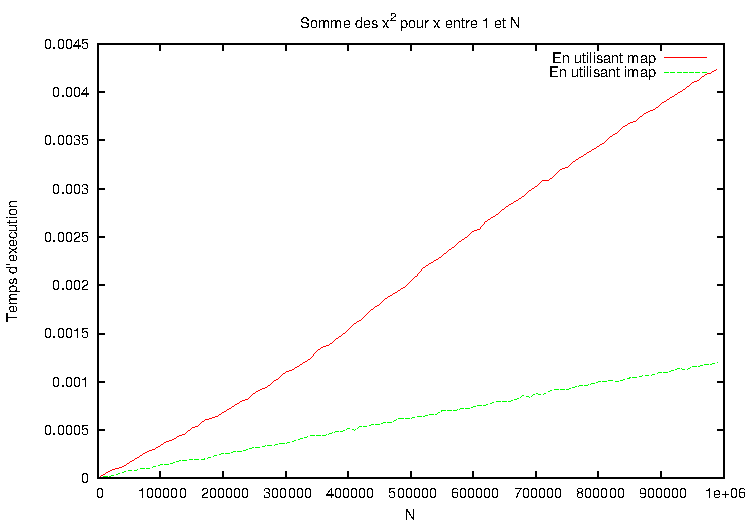
\includegraphics[width=\textwidth]{MapImap}
  \caption{Comparaison entre l'opérateur \texttt{map} et son itérateur équivalent.}
\end{figure}

\subsection*{Optimisations automatique de code}

Comme évoqué précédemment, le problème de la solution \texttt{itertools} est
qu'elle oblige le développeur python à choisir explicitement un
itérateur pour optimiser les performances. C'est pour cela qu'une
grande partie du projet a été dédiée à l'optimisation automatique du
programme initial pour utiliser des itérateurs quand cela est possible
et pertinent.

\vspace{.5em}

Les optimisations suivantes ont été implémentées :

\begin{itemize}
\item Transformation des opérateurs de base en itérateurs. Exemple :
  \texttt{map}->\texttt{imap}
\item Transformation des List Comprehension en iterateurs.
\item Transformation des Generator Expressions en itérateurs.
\end{itemize}

\vspace{.5em}

La plupart de ces optimisations se déroulent en deux parties :

\begin{enumerate}
\item Un algorithme analyse le programme pour détecter les parties
  pouvant bénéficier de l'optimisation.
\item Une transformation applique l'optimisation là où c'est possible.
\end{enumerate}

C'est la recherche et le développement d'algorithmes d'analyse qui a
été le plus couteux en temps étant donné la complexité du
problème. Les transformations quant à elles sont généralement plus
simples, voire triviales comme le remplacement de \texttt{map} par
\texttt{imap}.

Comme le montre la figure suivante, les optimisations ont permis un
gain en performance significatif quand elles sont possibles.

\begin{figure}[h]
  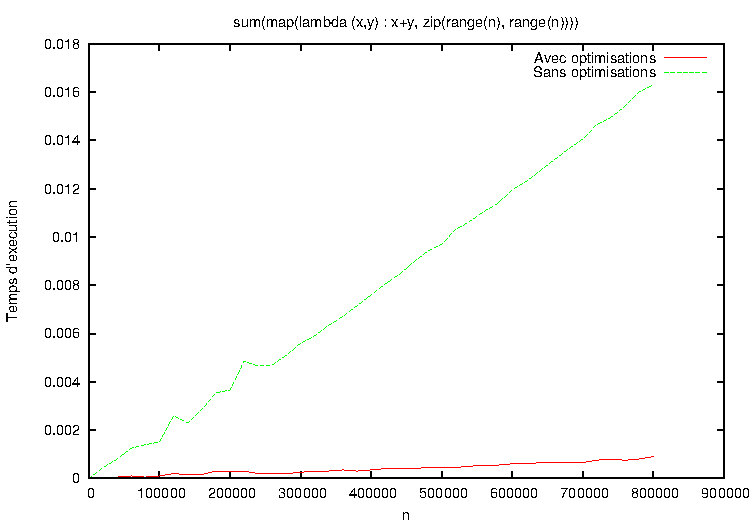
\includegraphics[width=\textwidth]{perf_optimization}
  \caption{Gain de performance dû aux optimisations.}
\end{figure}


\section*{Conclusion}

Les optimisations apportées par ce projet permettent à pythran
d'améliorer encore plus ses performances sur les cas qui s'y
prêtent. On doit cependant rappeler que cette optimisation ne porte
que sur les temps d'allocation de mémoire non nécessaire. Ces temps
peuvent être très importants dans des programme utilisant de nombreux
parcours de listes, mais ils peuvent être négligeables dans d'autres
types de programmes.

Les algorithmes développés pour analyser les cas propices aux
optimisations peuvent également être utiles à d'autres outils que
pythran. En particuliers, ils pourraient être utilisés par l'outil
2to3 pour faire de meilleurs choix de conversion. On gagnerait ainsi
en performance simplement en convertissant un programme python 2.7
vers python 3.

\end{document}

